\documentclass[UTF8,a4paper,12pt,fontset=fandol]{ctexart}

\usepackage{amsmath}
\usepackage{booktabs}
\usepackage{float}
\usepackage{geometry}
\usepackage{graphicx}
\usepackage{hyperref}
\usepackage{threeparttable}
\usepackage{url}

\geometry{left=2.6cm,right=2.6cm,top=2.6cm,bottom=2.6cm}
\graphicspath{{figures/}}
\hypersetup{hidelinks}
\linespread{1.25}

\title{基于重采样与生成式插补策略的大学英语教学质量评估模型研究}
\author{}
\date{}

\begin{document}
\maketitle

\begin{abstract}
大学英语教学质量评估数据通常具有明显的类别不平衡特征，尤其是高质量样本数量稀少，容易导致分类模型在总体准确率较高的同时忽略关键少数类。针对这一问题，本文以包含1650条样本的大学英语教学评价数据为研究对象，选取13维数值型学习行为与评价反馈特征，比较不采样、SMOTE、SMOTE-ENN、边界SMOTE和轻量表格GAN插补五类采样/插补策略在决策树、随机森林、支持向量机、K近邻和逻辑回归五种模型上的表现。实验采用5折分层交叉验证，并以高质量类F1、宏平均F1、G-均值和ROC/AUC作为评价指标。结果显示，逻辑回归与边界SMOTE组合在高质量类F1上取得最优结果（0.811），逻辑回归与SMOTE组合取得第二结果（0.801）；同时，SMOTE在高质量类召回率与G-均值上表现突出，主要逻辑回归组合在一对多ROC曲线中也保持较高AUC，说明过采样插值策略能够显著缓解极端类别不平衡造成的少数类识别不足。研究表明，在大学英语教学质量评估场景中，模型选择与采样/插补策略需要联合优化，不能仅依赖总体准确率判断模型有效性。
\end{abstract}

\noindent\textbf{关键词：}大学英语教学质量评估；类别不平衡；SMOTE；边界SMOTE；GAN插补；5折交叉验证

\section{引言}
随着教育信息化与学习分析技术的发展，教学质量评估逐渐从单一的主观评价转向多源数据驱动的综合建模。大学英语课程具有学习过程长、课堂互动频繁、线上线下行为并存等特点，学生出勤、作业完成、平台登录、视频学习、课堂参与以及教师反馈等数据能够从多个角度反映教学质量。然而，在真实评价数据中，高质量类别样本往往远少于中质量和低质量样本，形成极端类别不平衡问题。

在类别不平衡条件下，传统分类模型倾向于学习多数类分布，从而在整体准确率较高的情况下仍然难以识别少数类。对于大学英语教学质量评估而言，高质量教学样本的识别具有直接的教学诊断价值。如果模型无法稳定识别高质量类别，就难以为教学经验总结、课堂改进和质量保障提供可靠依据。因此，本文关注的核心问题是：在高质量样本极少的情况下，何种模型与采样/插补方式组合能够更有效地识别少数类教学质量样本。

本文在原有SMOTE、SMOTE-ENN和边界SMOTE比较的基础上，进一步补充轻量表格GAN生成式插补方法，并使用5折分层交叉验证重新评估不同模型与不同插补方式的组合表现。为避免准确率掩盖少数类识别失败，本文重点报告高质量类F1、宏平均F1和G-均值。

\section{数据与特征}
本文使用的大学英语教学质量评估数据集包含1650条样本。原始数据包括学生、课程、教师、学期等管理字段，以及出勤率、作业完成率、平均作业分数、考试分数、平均测验分数、参与频率、学习管理系统登录次数、平均会话时长、视频完成率、自我评估分数、同行反馈分数、教师反馈分数和参与度指数等数值型指标。为避免模型记忆具体学生、教师或课程批次，本文未将身份类字段作为预测变量，最终使用13维数值特征建模。

数据标签包括低质量、中质量和高质量三类。其中低质量样本852个，中质量样本759个，高质量样本仅39个，占总样本量的2.36\%。高质量类别与最大类别之间的不平衡比例超过20:1，属于典型的极端类别不平衡场景。本文保留三分类任务设定，而不是将高质量类别与其他类别合并，以便考察模型对稀缺但教学意义较强类别的识别能力。

\section{方法}
\subsection{采样/插补策略}
本文将重采样、基于插值的过采样以及生成式样本补充统一表述为采样/插补策略，并比较以下五类方法。

\textbf{不采样}直接使用原始训练集训练模型，用于观察类别不平衡对各类模型的基础影响。

\textbf{SMOTE}在少数类样本及其近邻之间进行线性插值，生成合成样本，从而提高少数类在训练集中的密度。其基本形式为
\begin{equation}
    x_{\mathrm{new}} = x_i + \lambda(x_j-x_i), \quad \lambda \in [0,1],
\end{equation}
其中$x_i$为少数类样本，$x_j$为同类近邻样本。

\textbf{边界SMOTE}优先选择位于决策边界附近的少数类样本进行插值扩增，重点增强容易被多数类覆盖的边界区域。

\textbf{SMOTE-ENN}先使用SMOTE生成合成样本，再使用编辑近邻规则清理边界噪声样本。该方法兼具过采样和欠采样特征，但在类别高度重叠时也可能删除有价值的边界样本。

\textbf{轻量表格GAN插补}面向高质量类别构建生成器与判别器，在少数类特征空间中生成补充样本。考虑到高质量训练样本数量极少，本文未将GAN样本扩增至多数类规模，而是采用适度扩增策略，以降低过度生成导致的边界假阳性风险。

\subsection{分类模型}
本文比较五种常用机器学习分类器：决策树、随机森林、支持向量机、K近邻和逻辑回归。决策树和K近邻对局部样本分布较敏感；随机森林通过集成学习降低单模型方差；支持向量机通过核函数刻画非线性边界；逻辑回归虽然形式较简单，但在高维标准化特征与插值样本共同作用下通常具有较好的稳定性。

\subsection{评价指标与验证方式}
实验采用5折分层交叉验证。每一折均先在训练折上拟合标准化器，再在训练折内部执行采样/插补操作，测试折不参与任何重采样过程，以避免数据泄漏。评价指标包括类别F1、宏平均F1、平衡准确率、G-均值以及一对多ROC曲线和AUC。ROC曲线基于各折测试集的折外预测分数绘制，用于检验模型在不同判别阈值下的区分能力。本文重点关注高质量类F1，其定义为
\begin{equation}
    F1 = \frac{2PR}{P+R},
\end{equation}
其中$P$为精确率，$R$为召回率。G-均值用于衡量多类别召回率的均衡性：
\begin{equation}
    G\text{-mean} = \left(\prod_{k=1}^{K} R_k \right)^{1/K}.
\end{equation}
当任一类别召回率接近0时，G-均值会显著下降，因此更适合反映不平衡分类中的结构性失败。

\section{实验结果}
表\ref{tab:cv-results}给出了五种模型与五类采样/插补策略组合下的5折交叉验证结果。每个单元格采用“均值$\pm$标准差”的形式表示，其中均值用于判断模型组合的整体效果，标准差用于反映不同折次之间的波动。表中各指标列的最优均值使用加粗标记，第二优均值使用下划线标记；模型与采样/插补方式名称的加粗或下划线依据高质量F1均值排序。

\begin{table}[htbp]
\centering
\caption{不同模型与采样/插补方式下的5折交叉验证结果（均值$\pm$标准差）}
\label{tab:cv-results}
\small
\setlength{\tabcolsep}{3.6pt}
\resizebox{\textwidth}{!}{%
\begin{tabular}{llcccc}
\toprule
模型 & 采样/插补方式 & 高质量F1 & 高质量召回率 & 宏平均F1 & G-均值 \\
\midrule
\textbf{逻辑回归} & \textbf{边界SMOTE} & \textbf{0.811$\pm$0.047} & \underline{0.975$\pm$0.056} & \textbf{0.923$\pm$0.017} & 0.974$\pm$0.019 \\
\underline{逻辑回归} & \underline{SMOTE} & \underline{0.801$\pm$0.059} & \textbf{1.000$\pm$0.000} & \underline{0.920$\pm$0.022} & \textbf{0.982$\pm$0.005} \\
逻辑回归 & GAN插补 & 0.793$\pm$0.113 & 0.818$\pm$0.172 & 0.918$\pm$0.041 & 0.919$\pm$0.066 \\
逻辑回归 & SMOTE-ENN & 0.761$\pm$0.045 & \textbf{1.000$\pm$0.000} & 0.901$\pm$0.018 & \underline{0.976$\pm$0.007} \\
逻辑回归 & 不采样 & 0.654$\pm$0.215 & 0.532$\pm$0.247 & 0.873$\pm$0.072 & 0.785$\pm$0.134 \\
支持向量机 & SMOTE & 0.620$\pm$0.162 & 0.557$\pm$0.197 & 0.842$\pm$0.055 & 0.789$\pm$0.101 \\
支持向量机 & 边界SMOTE & 0.616$\pm$0.172 & 0.561$\pm$0.178 & 0.842$\pm$0.060 & 0.794$\pm$0.088 \\
随机森林 & SMOTE-ENN & 0.600$\pm$0.143 & 0.589$\pm$0.163 & 0.801$\pm$0.048 & 0.777$\pm$0.070 \\
支持向量机 & SMOTE-ENN & 0.572$\pm$0.230 & 0.604$\pm$0.278 & 0.812$\pm$0.076 & 0.781$\pm$0.161 \\
随机森林 & SMOTE & 0.565$\pm$0.134 & 0.482$\pm$0.196 & 0.797$\pm$0.040 & 0.728$\pm$0.091 \\
随机森林 & 边界SMOTE & 0.555$\pm$0.176 & 0.457$\pm$0.220 & 0.800$\pm$0.062 & 0.718$\pm$0.116 \\
随机森林 & GAN插补 & 0.513$\pm$0.136 & 0.386$\pm$0.127 & 0.781$\pm$0.056 & 0.682$\pm$0.084 \\
支持向量机 & GAN插补 & 0.485$\pm$0.120 & 0.382$\pm$0.117 & 0.795$\pm$0.044 & 0.698$\pm$0.075 \\
决策树 & 边界SMOTE & 0.479$\pm$0.178 & 0.532$\pm$0.231 & 0.720$\pm$0.048 & 0.707$\pm$0.092 \\
决策树 & SMOTE-ENN & 0.474$\pm$0.058 & 0.589$\pm$0.137 & 0.689$\pm$0.024 & 0.713$\pm$0.053 \\
决策树 & 不采样 & 0.470$\pm$0.083 & 0.511$\pm$0.144 & 0.704$\pm$0.035 & 0.695$\pm$0.069 \\
决策树 & SMOTE & 0.468$\pm$0.115 & 0.561$\pm$0.092 & 0.706$\pm$0.035 & 0.720$\pm$0.041 \\
决策树 & GAN插补 & 0.457$\pm$0.170 & 0.486$\pm$0.156 & 0.705$\pm$0.050 & 0.686$\pm$0.057 \\
K近邻 & GAN插补 & 0.398$\pm$0.141 & 0.432$\pm$0.254 & 0.707$\pm$0.056 & 0.658$\pm$0.145 \\
K近邻 & 边界SMOTE & 0.319$\pm$0.072 & 0.821$\pm$0.141 & 0.656$\pm$0.033 & 0.797$\pm$0.049 \\
K近邻 & SMOTE & 0.301$\pm$0.048 & 0.846$\pm$0.054 & 0.647$\pm$0.022 & 0.801$\pm$0.022 \\
K近邻 & SMOTE-ENN & 0.262$\pm$0.040 & 0.846$\pm$0.054 & 0.621$\pm$0.021 & 0.782$\pm$0.028 \\
随机森林 & 不采样 & 0.089$\pm$0.122 & 0.050$\pm$0.068 & 0.636$\pm$0.044 & 0.189$\pm$0.259 \\
支持向量机 & 不采样 & 0.000$\pm$0.000 & 0.000$\pm$0.000 & 0.632$\pm$0.009 & 0.000$\pm$0.000 \\
K近邻 & 不采样 & 0.000$\pm$0.000 & 0.000$\pm$0.000 & 0.575$\pm$0.011 & 0.000$\pm$0.000 \\
\bottomrule
\end{tabular}
}%
\vspace{2pt}
\parbox{\textwidth}{\footnotesize 注：表中数值为5折交叉验证的均值$\pm$标准差，标准差按5折结果计算。各指标列中最优均值加粗，第二优均值加下划线；模型与采样/插补方式名称的加粗或下划线依据高质量F1均值排序。}
\end{table}


从高质量类F1看，逻辑回归+边界SMOTE取得最优结果，为0.811；逻辑回归+SMOTE位列第二，为0.801。两者均明显高于不采样条件下的逻辑回归结果0.654，说明边界插值和常规SMOTE均能显著提高高质量样本识别能力。逻辑回归+GAN插补的高质量F1为0.793，低于边界SMOTE和SMOTE，但高于其他大多数模型组合，表明生成式插补具有一定有效性，但在样本极少时仍需要谨慎控制生成规模。

图\ref{fig:high-f1}展示了不同模型在不同采样/插补方式下的高质量类F1箱线图。箱体反映5折交叉验证中各折结果的分布，白色圆点表示均值。逻辑回归在SMOTE、边界SMOTE和GAN插补下均保持较强表现；随机森林和支持向量机在不采样条件下对高质量类别识别不足，使用SMOTE类方法后明显改善；K近邻虽然在采样后召回率提升，但精确率下降较明显，导致高质量F1仍然偏低。

\begin{figure}[H]
    \centering
    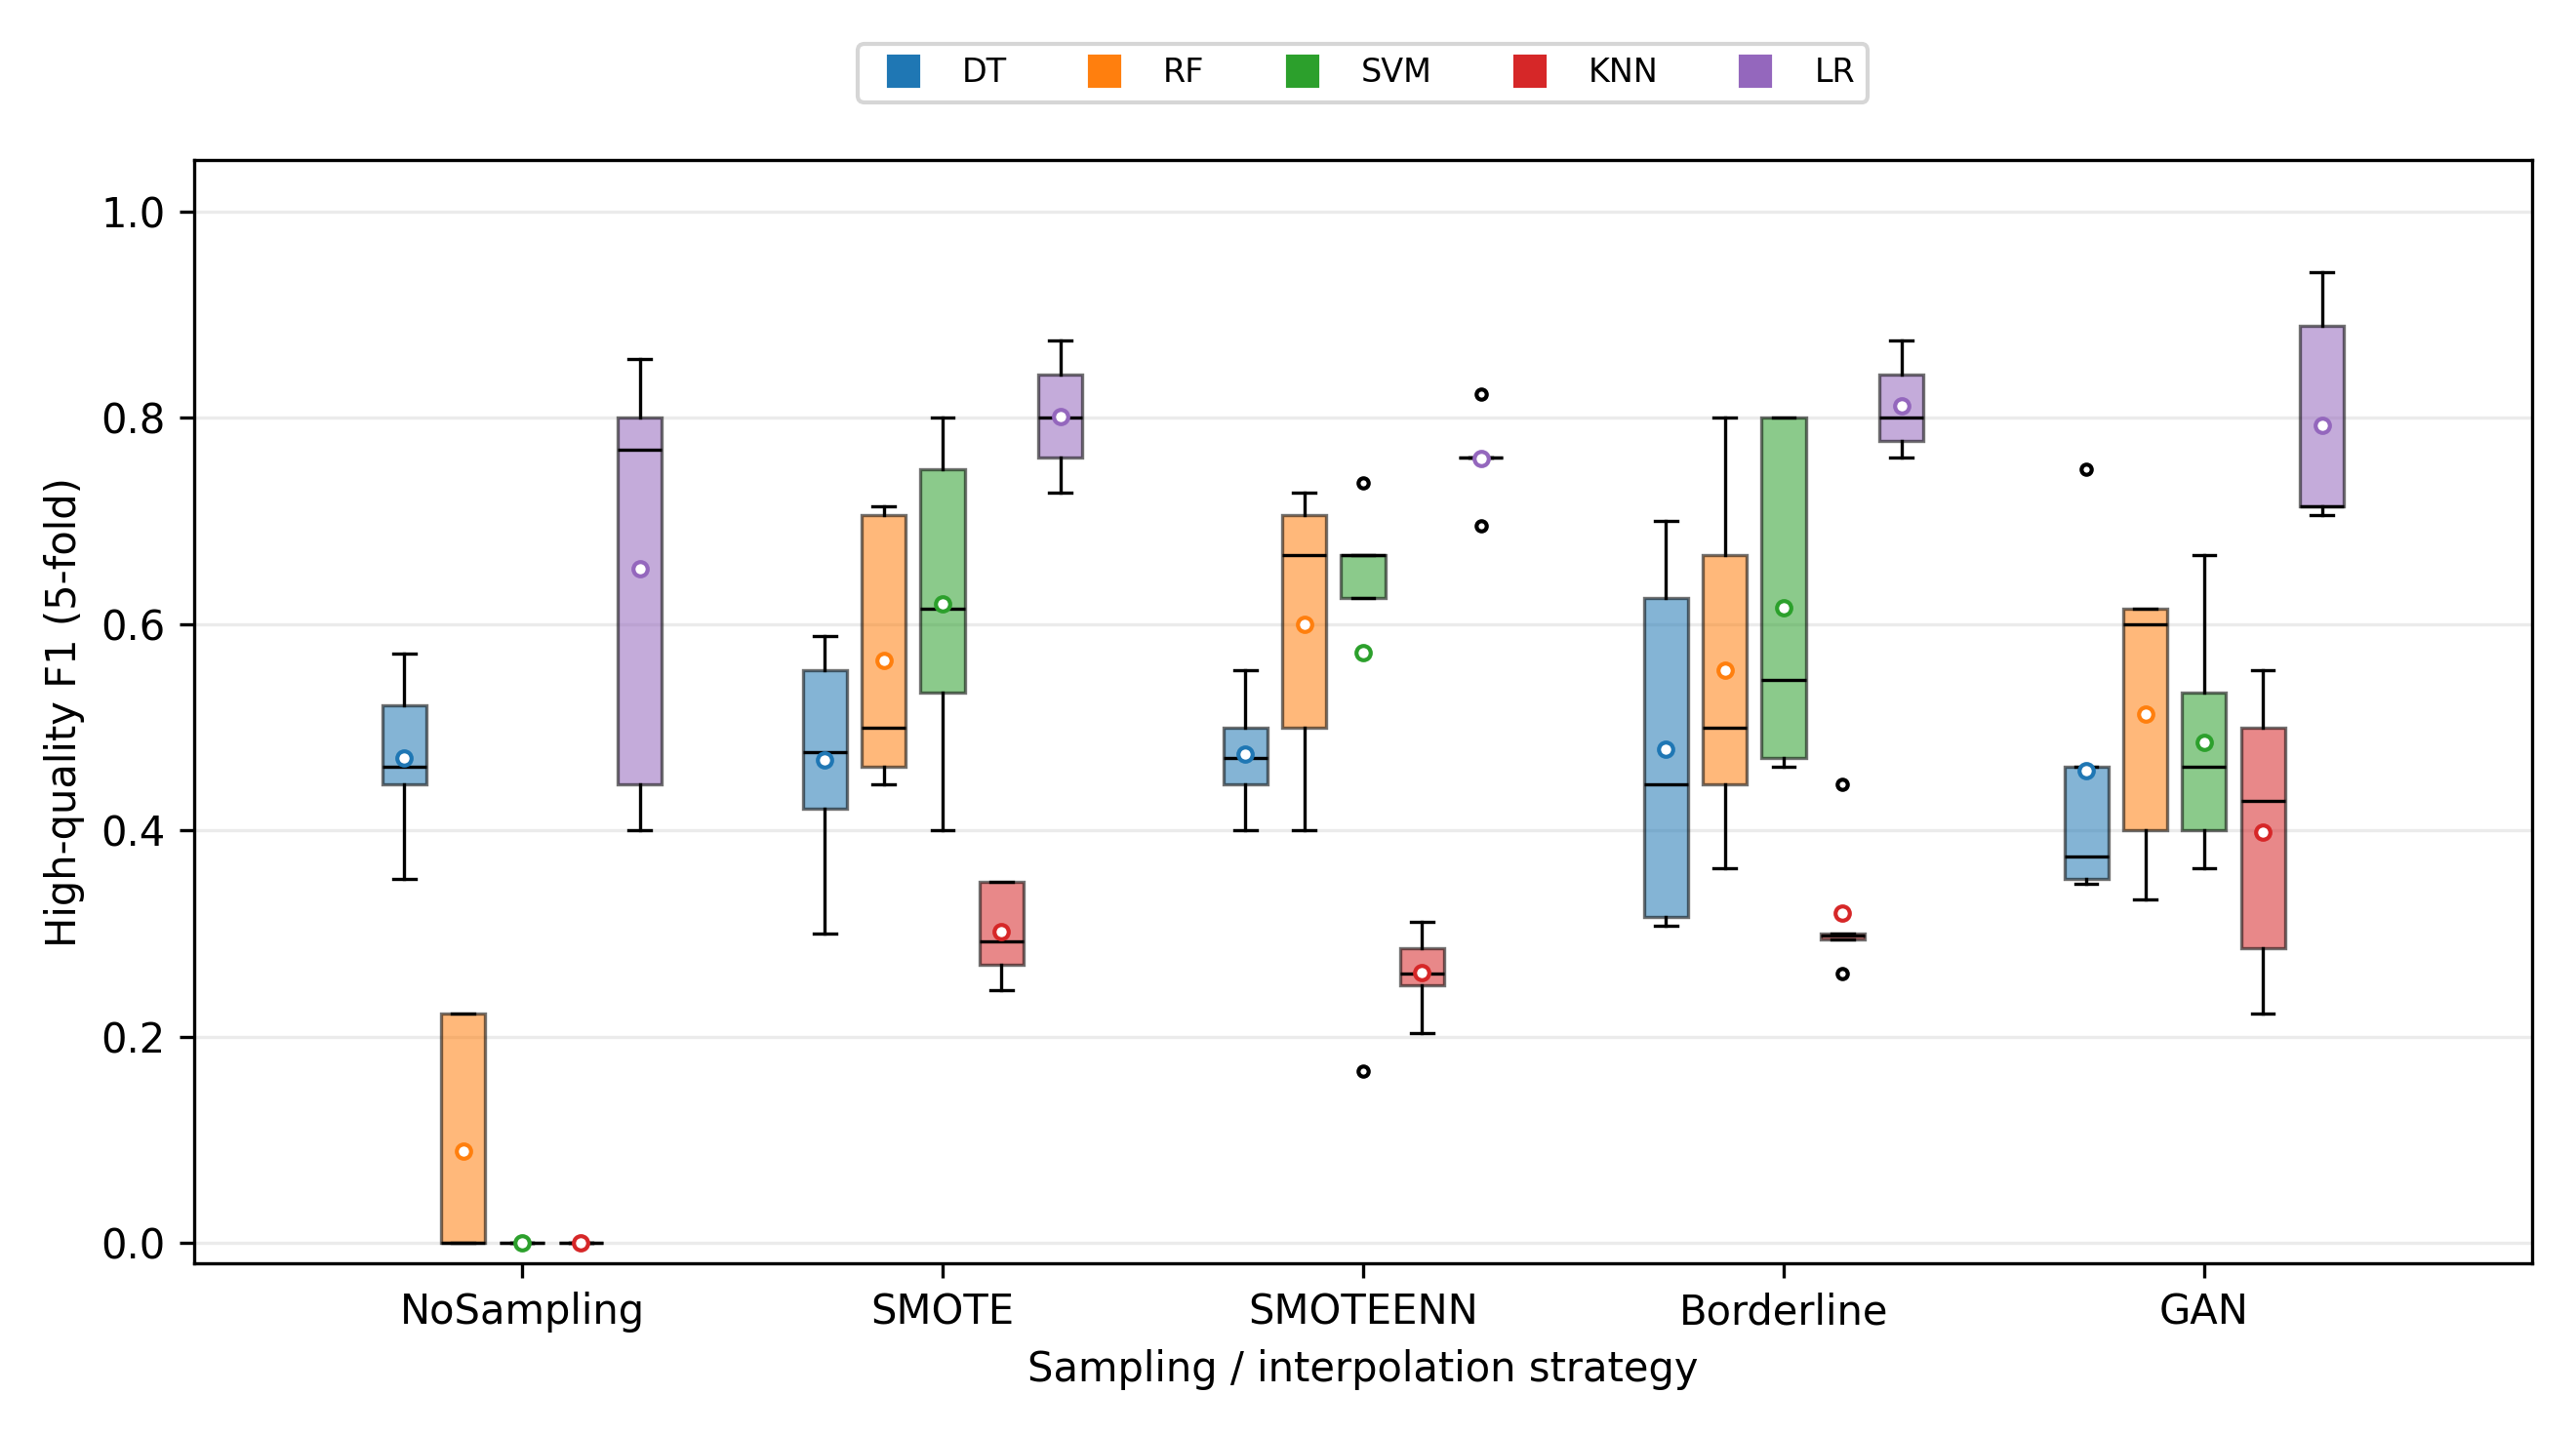
\includegraphics[width=0.92\textwidth]{cv_box_high_f1.png}
    \caption{不同模型在不同采样/插补方式下的高质量类F1箱线图（5折交叉验证）}
    \label{fig:high-f1}
\end{figure}

图\ref{fig:macro-f1}显示了宏平均F1的箱线图。逻辑回归在多数采样/插补方式下仍保持优势，说明其不仅提高了高质量类别识别能力，也没有显著牺牲中质量和低质量类别的整体表现。相比之下，K近邻在SMOTE-ENN等方法下虽然提升了少数类召回率，但宏平均F1仍受多数边界误判影响。

\begin{figure}[H]
    \centering
    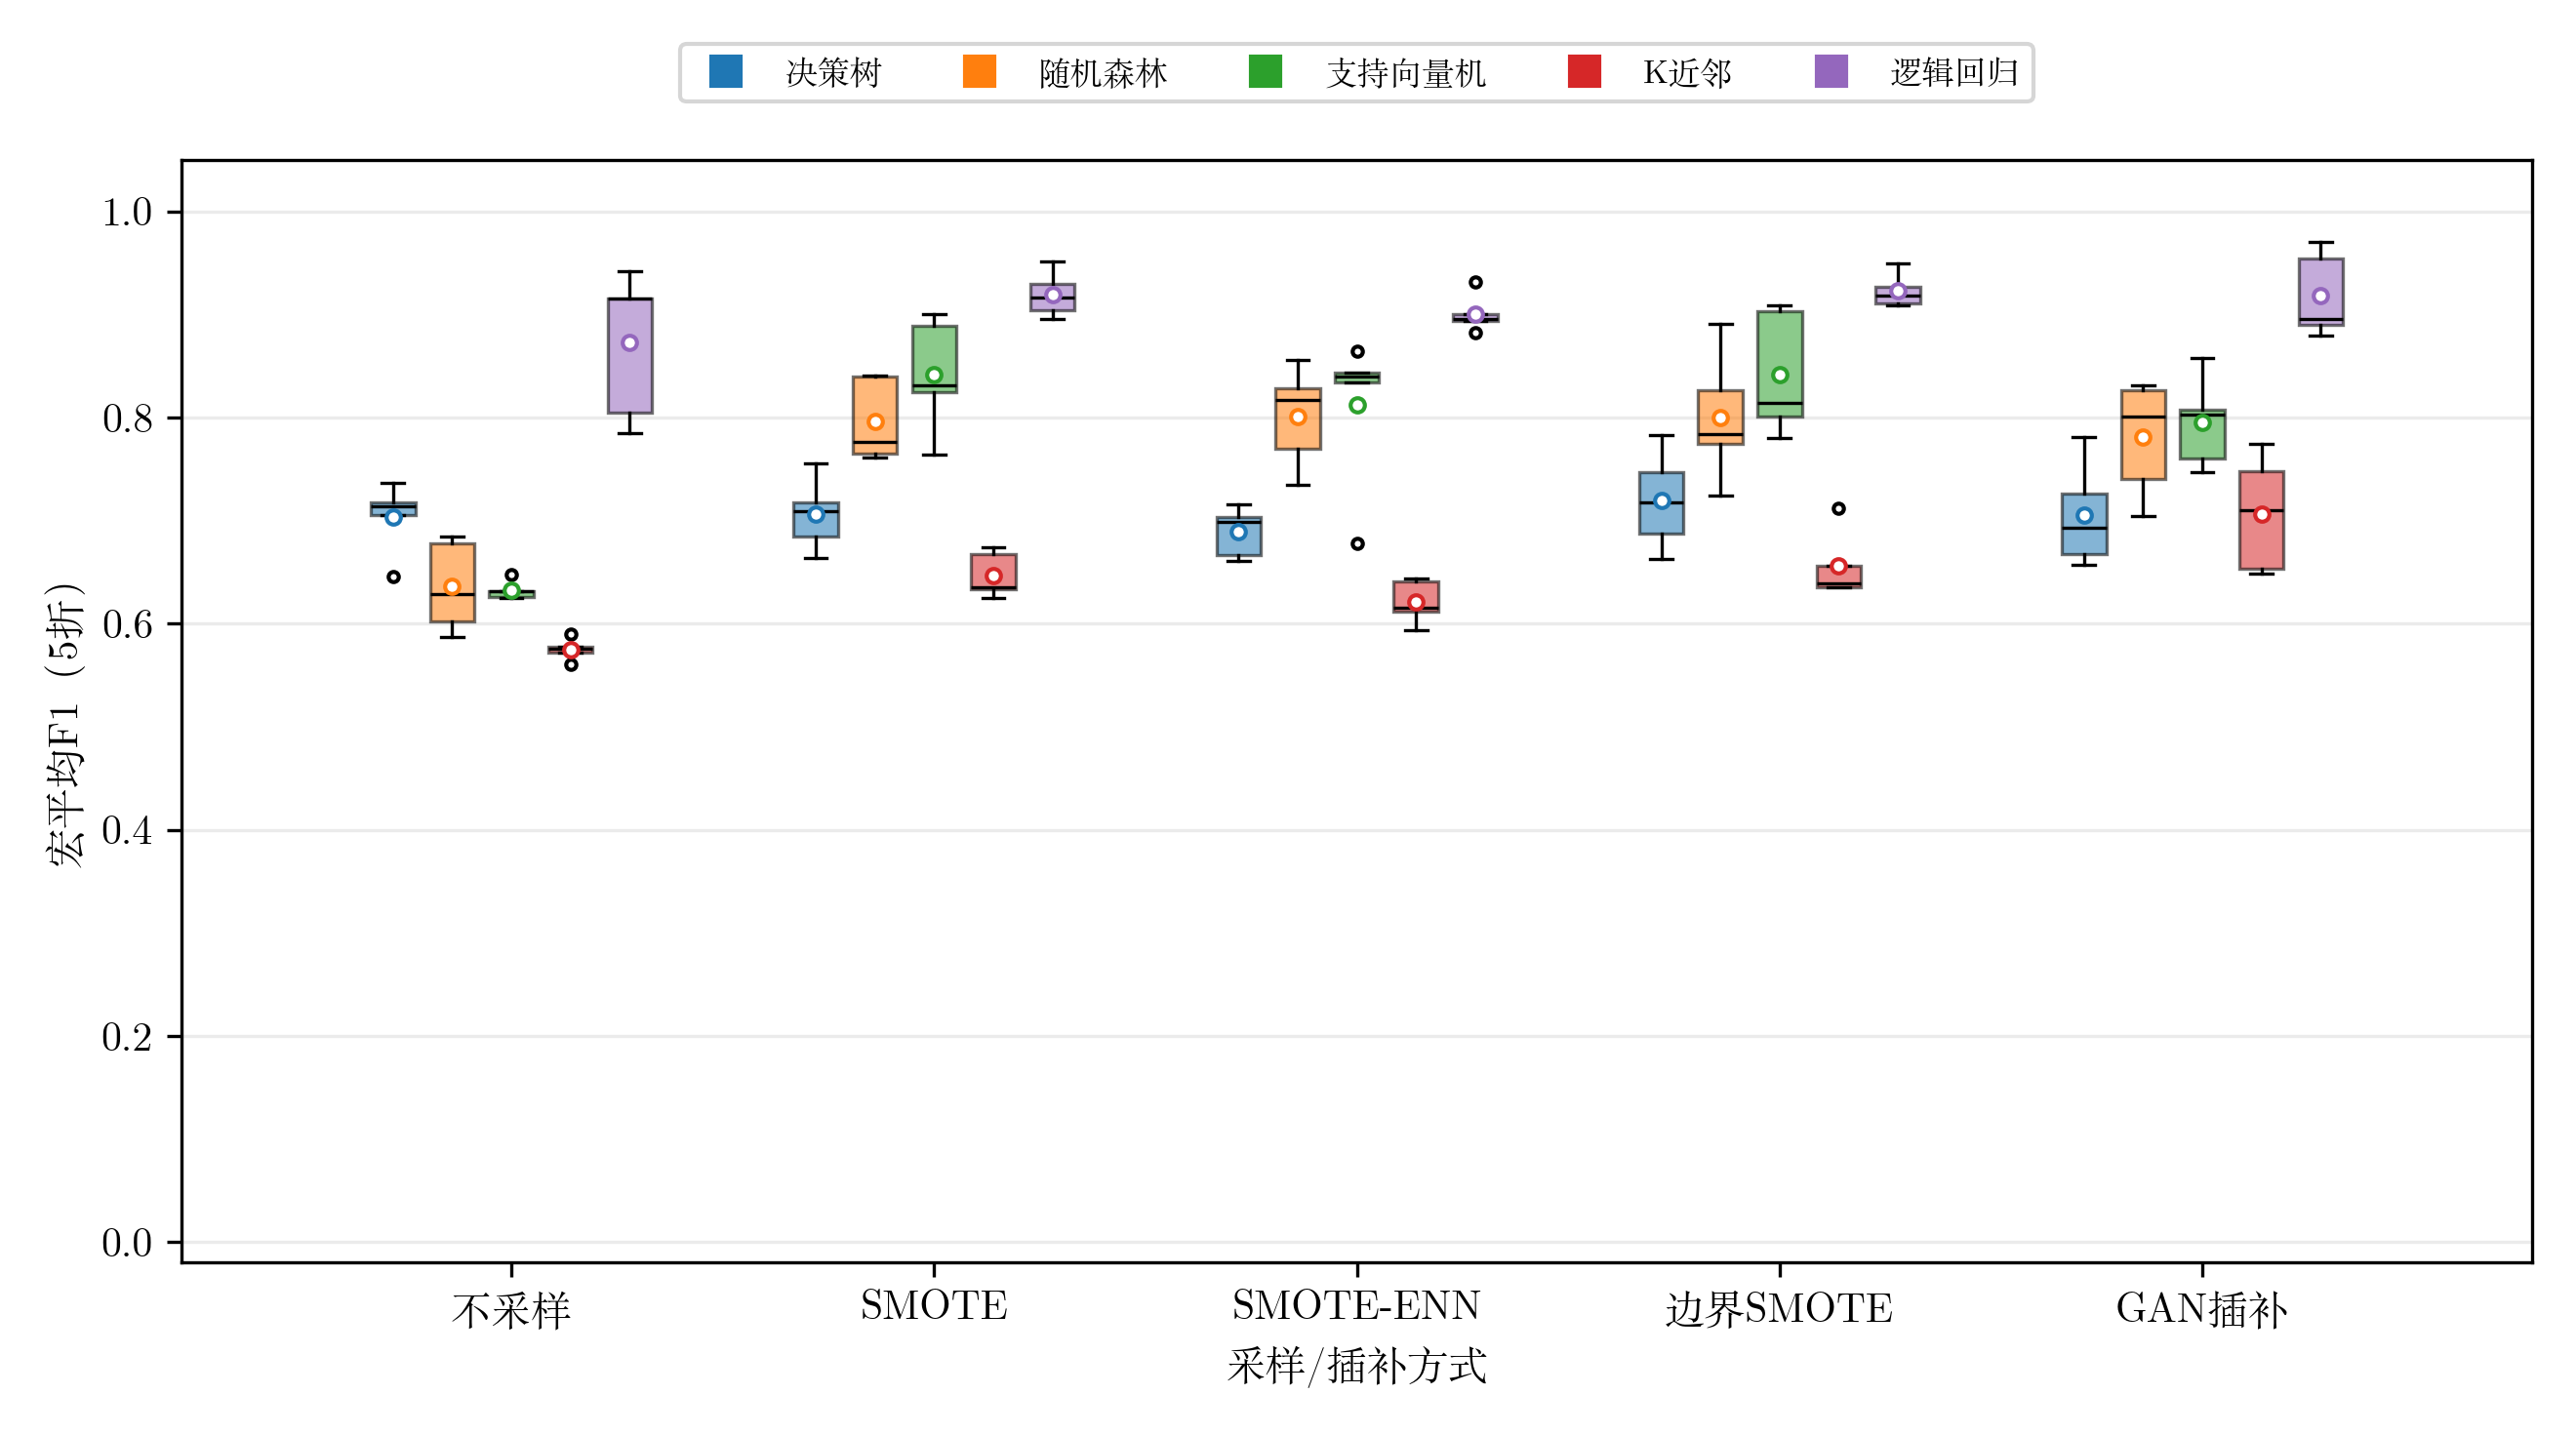
\includegraphics[width=0.92\textwidth]{cv_box_macro_f1.png}
    \caption{不同模型在不同采样/插补方式下的宏平均F1箱线图（5折交叉验证）}
    \label{fig:macro-f1}
\end{figure}

图\ref{fig:gmean}给出了G-均值箱线图。逻辑回归+SMOTE的G-均值均值最高，为0.982；逻辑回归+SMOTE-ENN位列第二，为0.976。该结果表明，如果研究目标更强调各类别召回率均衡，SMOTE和SMOTE-ENN具有较强优势；如果更强调高质量类F1的精确率与召回率折中，边界SMOTE更优。

\begin{figure}[H]
    \centering
    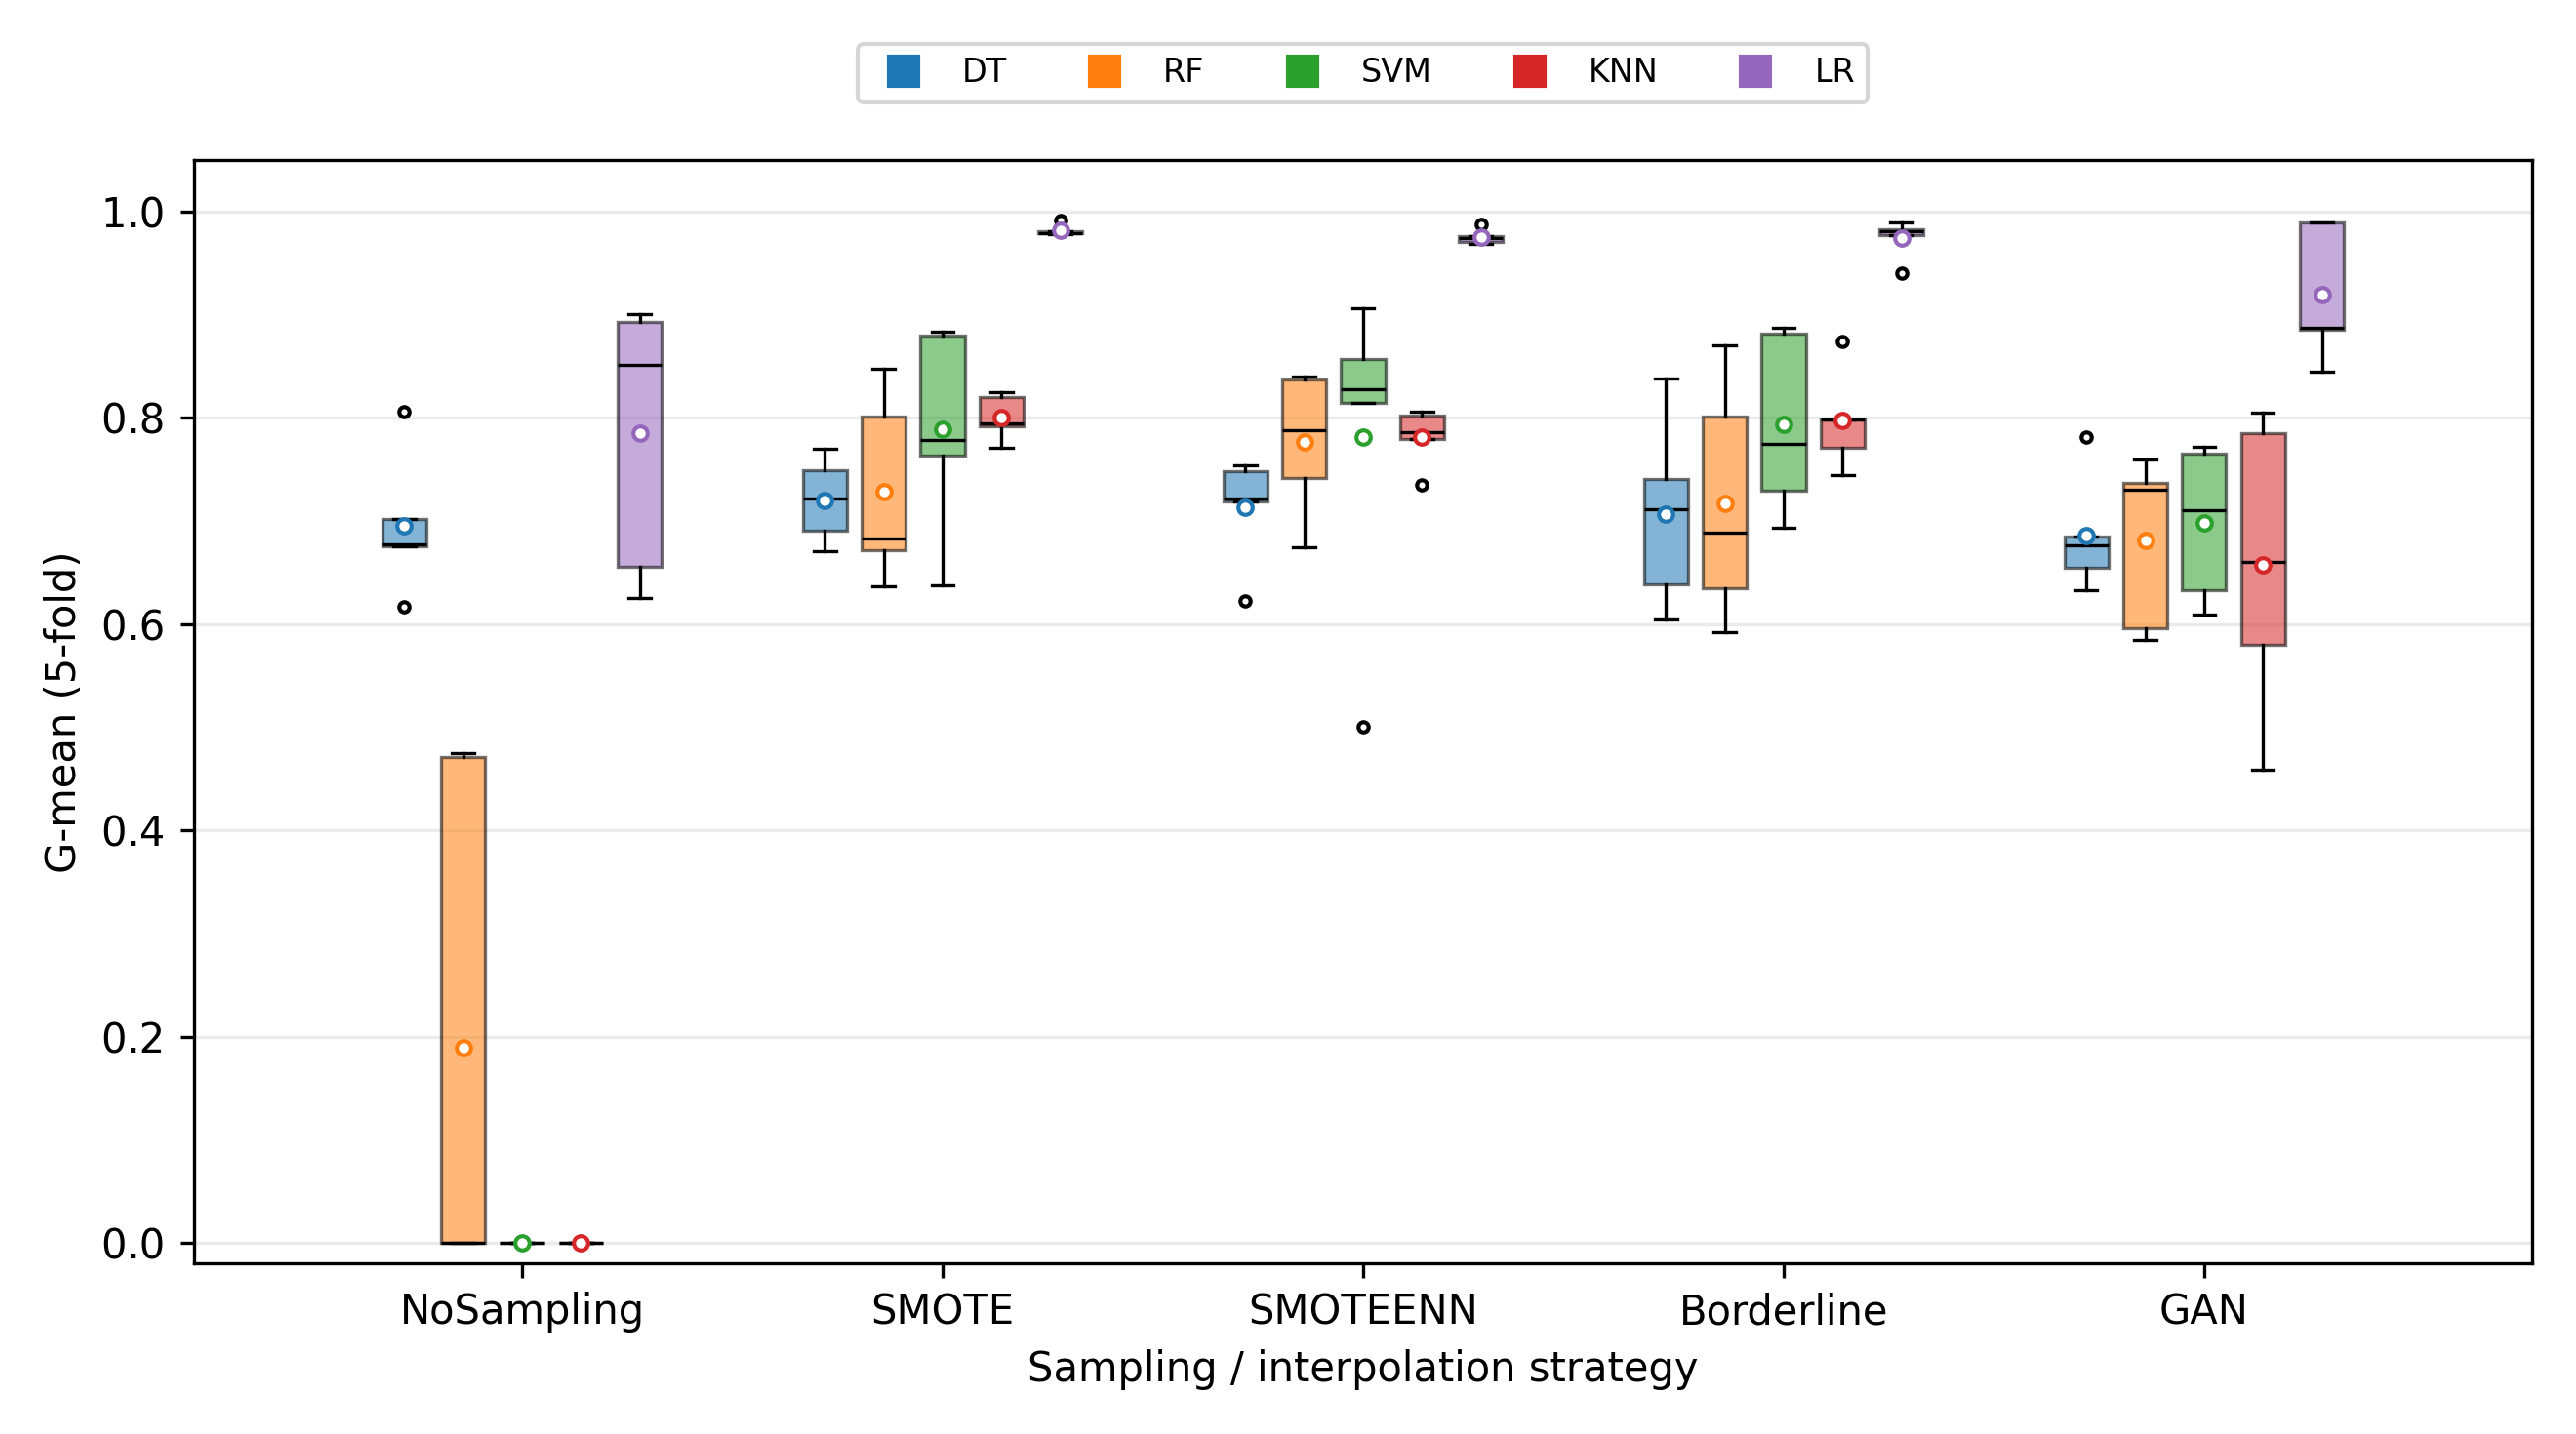
\includegraphics[width=0.92\textwidth]{cv_box_gmean.png}
    \caption{不同模型在不同采样/插补方式下的G-均值箱线图（5折交叉验证）}
    \label{fig:gmean}
\end{figure}

为进一步分析模型在不同阈值下的稳定性，本文基于5折交叉验证的折外预测分数绘制一对多ROC曲线。图\ref{fig:roc}展示了高质量、中质量和低质量三个类别的ROC结果。为避免曲线过密，图中仅展示高质量F1均值排名前6的模型组合，并在图例中标注AUC。结果显示，逻辑回归与SMOTE类采样/插补策略在三个类别上均具有较高AUC，其中高质量类别AUC最高接近0.999，说明这些组合不仅在固定分类阈值下具有较高F1，也能在阈值变化时保持较强区分能力。

\begin{figure}[H]
    \centering
    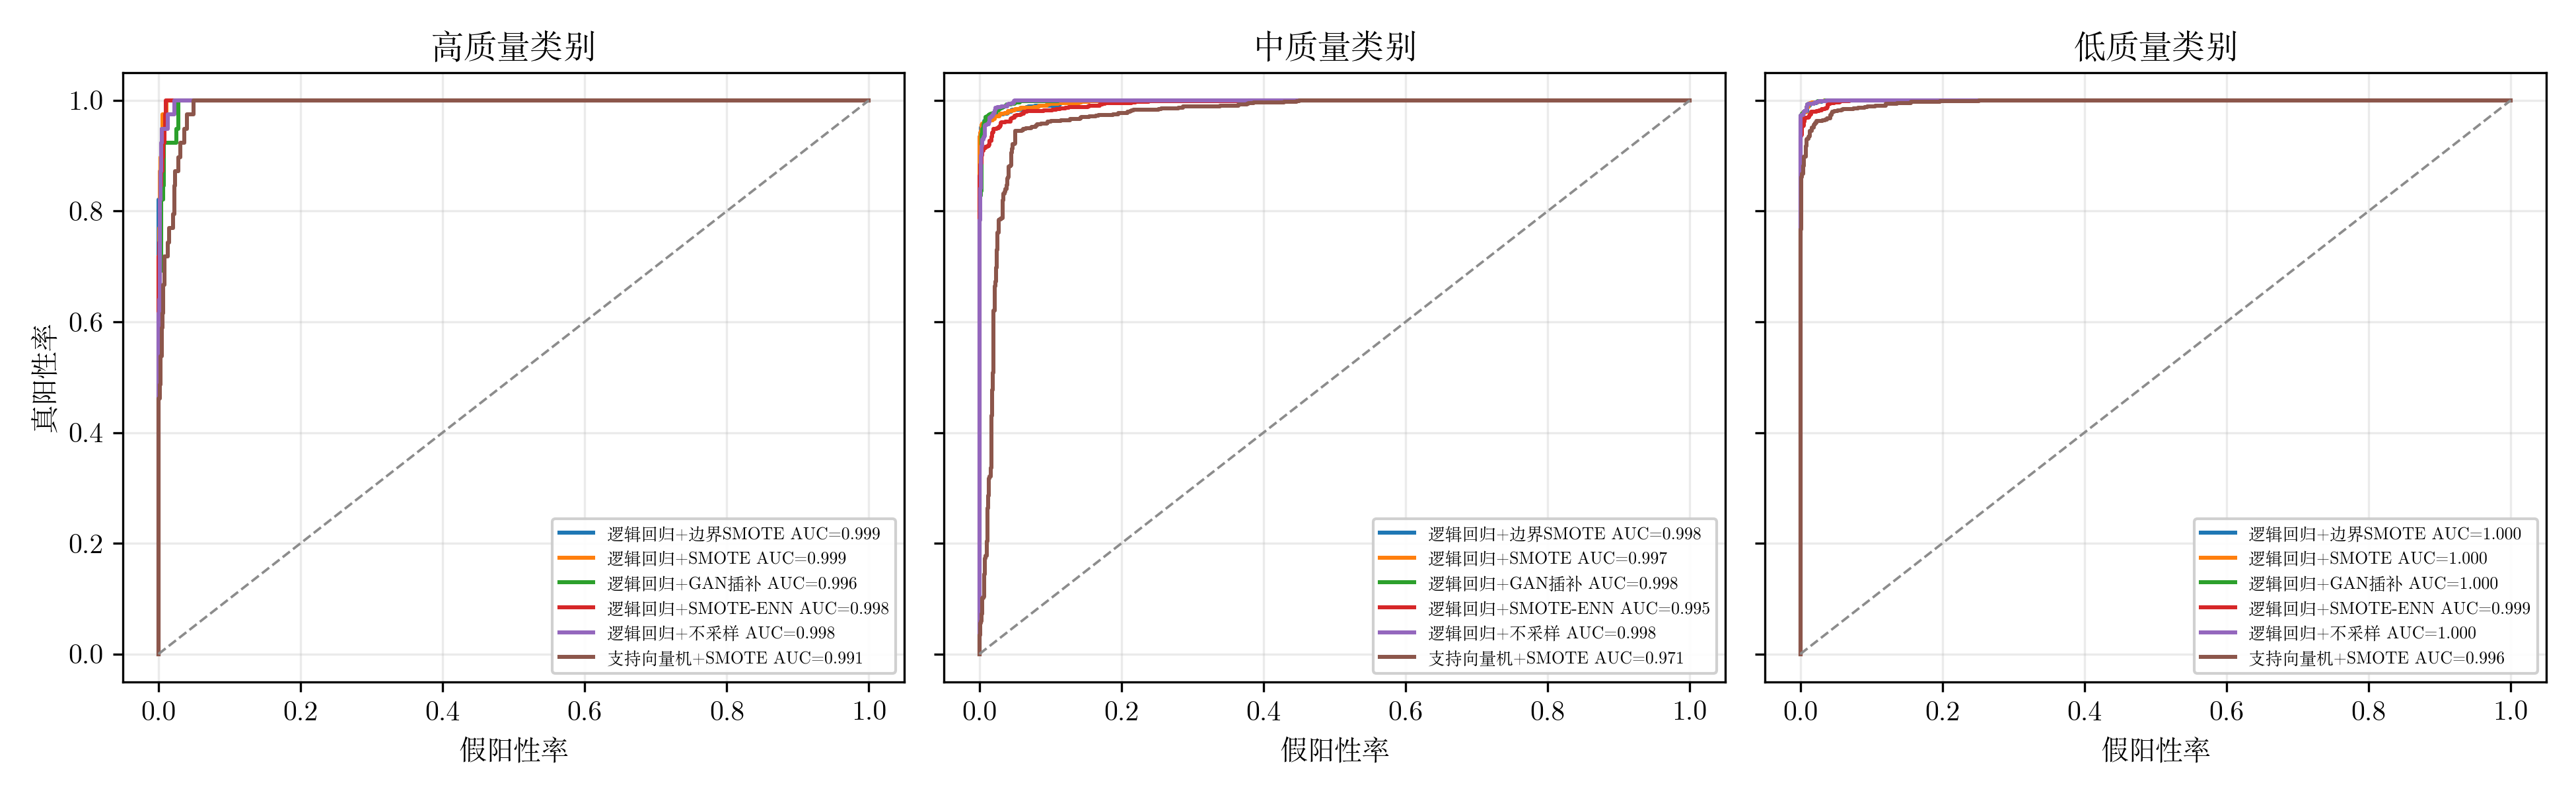
\includegraphics[width=\textwidth]{cv_roc_top_combinations.png}
    \caption{高质量F1排名前6模型组合的一对多ROC曲线（5折交叉验证折外预测分数）}
    \label{fig:roc}
\end{figure}

\section{讨论}
实验结果说明，大学英语教学质量评估中的高质量类别识别并非单纯依赖更复杂模型即可解决。随机森林和支持向量机在多数情况下具有较强分类能力，但在高质量样本极少时，如果缺少合适的采样/插补策略，仍容易出现少数类召回不足。逻辑回归在标准化特征和插值样本支持下表现稳定，说明当特征本身能够反映学习行为差异时，较简单的线性模型也可以取得较好的少数类识别结果。

边界SMOTE在高质量F1上的优势表明，高质量样本更可能分布在中质量样本附近的边界区域，而不是形成完全独立的特征簇。大学英语教学中的高质量课堂往往表现为出勤、作业、平台学习、互动反馈等多项指标的综合改善，因此其特征空间与中质量课堂存在重叠。针对边界样本进行重点插值，有助于模型更清楚地学习高质量与中质量之间的判别边界。

GAN插补在本实验中取得了较高但并非最优的高质量F1。原因可能在于高质量训练样本数量过少，生成模型难以充分学习少数类内部的多样性；同时，若生成样本过多，可能会扩大高质量类别的边界并增加误判。因此，在教育数据挖掘的小样本不平衡场景中，生成式插补应作为补充方法，并与分层交叉验证、错分样本分析共同报告。

\section{结论}
本文使用LaTeX重写并重新组织了大学英语教学质量评估中的类别不平衡研究，补充了完整的5折分层交叉验证实验。结果表明，逻辑回归+边界SMOTE在高质量类F1上表现最优，逻辑回归+SMOTE表现第二；若以G-均值衡量类别召回均衡性，逻辑回归+SMOTE最优。ROC/AUC结果进一步表明，排名靠前的逻辑回归与SMOTE类组合在阈值变化下仍具有较强区分能力。总体来看，采样/插补方式对少数类识别能力具有决定性影响，大学英语教学质量评估模型应优先报告高质量类F1、宏平均F1、G-均值和ROC/AUC，而不应仅依据总体准确率判断模型优劣。

后续研究可进一步引入更稳定的条件表格GAN、扩散模型或代价敏感学习方法，并结合课程教学专家知识对错分样本进行解释，从而提升模型在真实教学质量保障场景中的可用性。

\begin{thebibliography}{99}
\bibitem{han2005borderline}
Han H, Wang W Y, Mao B H. Borderline-SMOTE: A new over-sampling method in imbalanced data sets learning[C]. International Conference on Intelligent Computing, 2005: 878--887.

\bibitem{chawla2002smote}
Chawla N V, Bowyer K W, Hall L O, et al. SMOTE: Synthetic minority over-sampling technique[J]. Journal of Artificial Intelligence Research, 2002, 16: 321--357.

\bibitem{batista2004study}
Batista G E A P A, Prati R C, Monard M C. A study of the behavior of several methods for balancing machine learning training data[J]. ACM SIGKDD Explorations Newsletter, 2004, 6(1): 20--29.

\bibitem{xu2019ctgan}
Xu L, Skoularidou M, Cuesta-Infante A, et al. Modeling tabular data using conditional GAN[C]. Advances in Neural Information Processing Systems, 2019.

\bibitem{engelmann2020cwgan}
Engelmann J, Lessmann S. Conditional Wasserstein GAN-based oversampling of tabular data for imbalanced learning[J]. Expert Systems with Applications, 2021, 174: 114582.

\bibitem{gradstein2022gan}
Gradstein L, Yogev N, Lipshitz A, et al. Imbalanced classification via a tabular translation GAN[J]. Applied Soft Computing, 2022, 118: 108459.
\end{thebibliography}

\end{document}
